\chapter*{Apéndice: Poema de Navidad}
\addcontentsline{toc}{chapter}{Apéndice: Poema de Navidad}
\markboth{Apéndice: Poema de Navidad}{Apéndice: Poema de Navidad}
\vspace{0.3cm}
\begin{center}
\nopagebreak
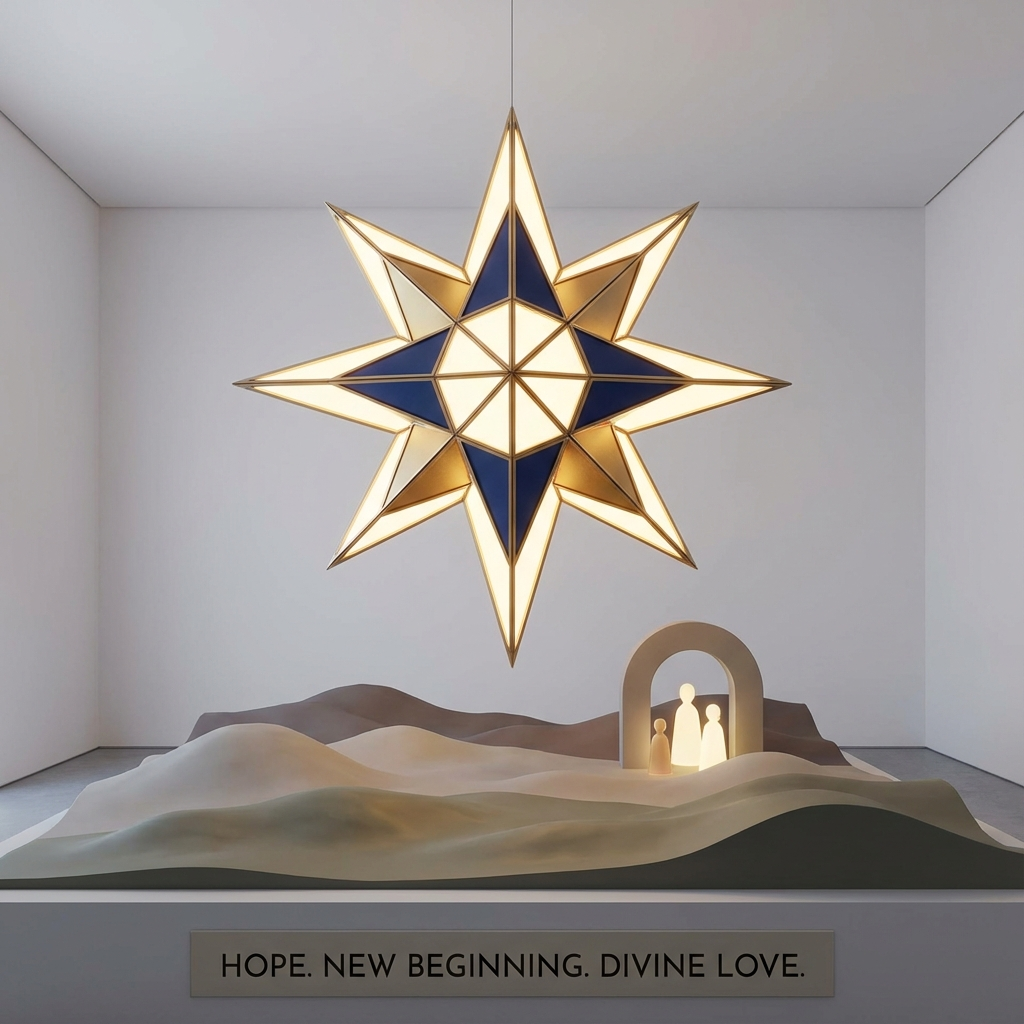
\includegraphics[width=0.45\textwidth,cfbox=gray!60 0.6pt 3pt]{christmas_star_modern.png}\\
\vspace{3pt}
{\small\itshape Estrella de Navidad: la luz que nace en el corazón.}
\end{center}

\vspace{0.4cm}
{\centering
\textbf{Navidad de Alta Frecuencia} \\
\textit{Por Maria Paz Arés Osset}

\vspace{0.4cm}

No busques al Niño en la paja fría de un tiempo remoto, \\
ni en el eco de un villancico que el viento ha roto. \\
No lo busques en la Gran Vía, bajo luces de neón, \\
donde el alma se vende barata en cada rincón.

\vspace{0.4cm}

Búscalo en el silencio que vibra en tu pecho, \\
en el templo sagrado que el Amor ha hecho. \\
Porque Jesús no lleva corona, ni oro, ni manto, \\
lleva vaqueros gastados y seca tu llanto.

\vspace{0.4cm}

Camina por Madrid, entre prisas y ruido, \\
un viajero eterno, por nadie temido. \\
Se sienta en Callao, te mira y sonríe: \\
«¿Por qué corres tanto? Párate y ríe.»

\vspace{0.4cm}

«La Navidad no es fecha, ni cena, ni regalo, \\
es vibrar tan alto que olvides lo malo. \\
Es saber que el pesebre no es madera ni heno, \\
es tu propio corazón, de esperanza lleno.»

\vspace{0.4cm}

Si vibras en miedo, si vibras en ira, \\
el Niño no nace, la estrella no brilla. \\
Pero si perdonas, si abrazas, si amas, \\
enciendes en ti las más puras llamas.

\vspace{0.4cm}

No nos dejes caer en la tentación de la tristeza, \\
levanta la vista, contempla la belleza. \\
Desde Las Rozas al cielo, de Colmenarejo al mar, \\
la única misión es aprender a Amar.

\vspace{0.4cm}

Líbranos del peso de vibrar en el suelo, \\
y danos las alas para alzar el vuelo. \\
Porque el Reino es ahora, la Gloria es hoy, \\
y en cada latido, contigo yo estoy.

\vspace{0.4cm}

Así que celebra, amigo, no el día marcado, \\
sino el Cristo viviente que tienes al lado. \\
Vibra alto, muy alto, que el mundo lo sienta, \\
que tu luz sea el faro en la gran tormenta.

\vspace{0.4cm}

Esta es la Navidad: no un cuento pasado, \\
sino el milagro eterno de haber despertado.
\par}


\vspace{1.5cm}
\begin{center}
\textit{Para completar esta experiencia vibracional, te invito a seguir los enlaces y sumergirte en la música del libro.}\\
\vspace{1cm}
\begin{minipage}{0.45\textwidth}
\centering
\qrcode[height=3.2cm]{https://open.spotify.com/album/6FkbQuY2d7F09zmG2hqnFK}\\
\vspace{0.4cm}\textbf{Escuchar en Spotify}
\end{minipage}\hfill
\begin{minipage}{0.45\textwidth}
\centering
\qrcode[height=3.2cm]{https://pazaresosset.es}\\
\vspace{0.4cm}\textbf{pazaresosset.es}
\end{minipage}
\end{center}